\chapter{Periferiche}
\section{I/O nel nucleo}  
\paragraph{Esempio} Ripartiamo dall'esempio visto quando abbiamo introdotto le interruzioni.
\begin{center}
	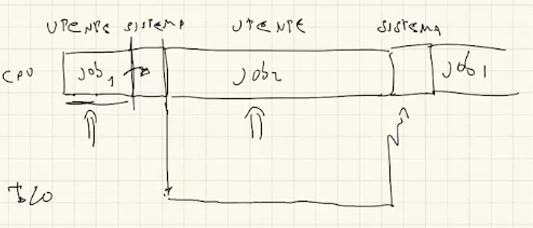
\includegraphics[scale=.8]{img/277.PNG}
\end{center}
\begin{itemize}
	\item Siamo in un sistema  batch, caratterizzato da \emph{job}. Avevamo preso come riferimento la \emph{Calcolatrice Elettronica Pisana}.
	\item \textbf{Abbiamo un job che a un certo punto deve fare un'operazione di I/O}. Invece di tenere occupata la CPU fino al termine dell'operazione chiamiamo una primitiva: questa esegue una routine di sistema che avvia l'operazione di I/O e cede la CPU a un altro \emph{job}. L'elemento fondamentale è che non serve la CPU (salvo casi rari) per portare a terminare l'operazione di I/O.
	\item Quando l'operazione di I/O finisce viene lanciata un'interruzione. Il \emph{job} in esecuzione viene interrotto e una routine di sistema ci riporta al primo \emph{job}, che adesso ha gli elementi per poter proseguire.
\end{itemize}
Dal punto di vista del \emph{job} l'operazione di I/O è istantanea: quello che abbiamo fatto è sospendere il \emph{job} e recuperarlo solo dopo aver completato l'operazione di I/O. Quello che è successo tra l'avvio e la conclusione dell'operazione è come se non fosse mai avvenuto (ripeto, dal punto di vista del job). 
\paragraph{Nel nostro caso} \[\boxed{\text{Job} = \text{Processo}}\]

\subsection{Limitazioni sull'utente} Come sempre non possiamo fidarci dell'utente, quindi
\begin{enumerate}
	\item impediamo all'utente l'accesso diretto alle periferiche, e
	\item forniamo all'utente delle primitive per svolgere le operazioni di I/O sotto il controllo del sistema
\end{enumerate} 
Il punto (1) lo otteniamo intervenendo sull'IOPL, nel registro dei flag. Questa cosa limita l'accesso solo alle periferiche con indirizzi nello spazio di I/O. Per quanto riguarda le periferiche con indirizzi nello spazio di memoria interveniamo con la MMU: facciamo in modo che lo spazio di indirizzamento virtuale non permetta di raggiungere, agli utenti, i frame relativi alle periferiche (poniamo il bit U/S a zero). 

\subsection{Questioni/problemi delegati alle primitive}
\begin{itemize}
	\item \textbf{Problema di \emph{mutua esclusione}}.
	
	L'utente non si preoccupa che la periferica con cui vuole dialogare non sia già occupata da qualcun altro. Supponiamo che il \emph{job} lanciato dalla routine dopo il primo \emph{job} voglia anch'esso rivolgersi alla periferica: siamo obbligati ad attendere che la tastiera abbia finito. 
	
	\item \textbf{Problema di \emph{sincronizzazione}}.
	
	Il job iniziale deve essere "risvegliato" solo dopo aver concluso l'operazione di I/O. 
\end{itemize} 

\subsection{Schema di una primitiva di I/O (IN read, OUT write)} La schematizzazione di un'operazione di I/O è un trasferimento di un certo numero di byte da e verso una periferica
\paragraph{Primitiva per periferica IN} Possiamo immaginarci una primitiva del seguente tipo
\begin{verbatim}
	read_n(int id, char* buf, natq quanti)
\end{verbatim}
l'utente che invoca la primitiva dovrà indicare: 
\begin{itemize}
	\item un qualcosa che identifichi la periferica da cui vuole leggere,
	\item dove i byte devono essere trasferiti,
	\item quanti byte devono essere trasferiti.
\end{itemize}  
La primitiva avvia un'operazione di ingresso dalla periferica ID: i \emph{quanti} byte letti dovranno trovarsi in memoria a partire dall'indirizzo \emph{buf} (nel buffer).

\paragraph{Primitiva per periferica OUT}
Lo schema non è molto diverso da quello già visto.
\begin{verbatim}
	write_n(int id, const char* buf, natq quanti)
\end{verbatim} 
\begin{itemize}
	\item Passiamo l'indirizzo del primo byte che si vuole scrivere sulla periferica (solo lettura, quindi può essere \emph{const}) e il numero di byte da  trasferire.
	\item La primitiva avvia un'operazione di uscita: poniamo il contenuto del buffer (cioè i \emph{quanti} byte dall'indirizzo \emph{buf}) nella periferica \emph{id}. 
\end{itemize}





\subsection{Necessità di più interruzioni, primitive e driver}
\begin{center}
	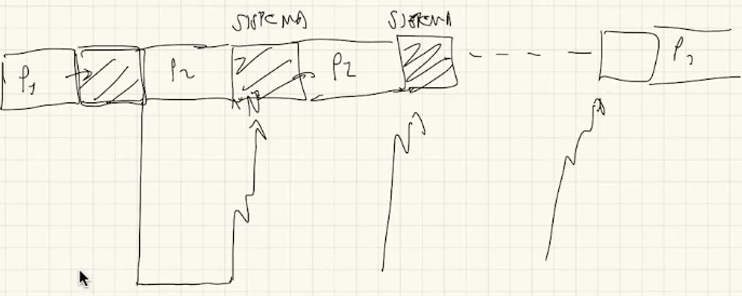
\includegraphics[scale=.7]{img/278.PNG}
\end{center}
Non è detto che un'operazione di I/O si risolva con una sola interruzione. Supponiamo di voler leggere un certo numero di byte dalla periferica: questa è in grado di inviarci un solo byte alla volta.  Questo significa che dovremo attendere per ogni byte, ricevendo più interruzioni (una ogni volta che un byte viene reso disponibile). 
\begin{itemize}
	\item Nel processo $P1$ lanciamo una routine di sistema con l'istruzione \emph{INT}. Questa avvia l'operazione di I/O e lascia la palla al processo $P2$.
	\item Il processo $P2$ continua finchè non riceve un'interruzione esterna: a quel punto si ritorna nella routine di sistema, si legge il byte e lo si pone da qualche parte.
	\item Dopo la lettura non ritorno subito nel processo $P1$, ma continuo ad eseguire il processo $P2$ (o un altro processo nel caso $P2$ sia concluso). 
\end{itemize} 
\begin{framed}
	\noindent Quello che andremo a fare è un'operazione eseguita in parte da una \textbf{primitiva} e in parte da un \textbf{driver}.
	\begin{itemize}
		\item La \emph{primitiva} avvia l'operazione di I/O e blocca il processo.
		\item Il \emph{driver} si occupa di trasferire effettivamente i byte e sbloccare il processo quando l'operazione si è conclusa.
	\end{itemize}
	Nell'implementazione dobbiamo risolvere la mutua esclusione e la sincronizzazione: lo facciamo \textbf{utilizzando i semafori}. 
	\begin{itemize}
		\item Per la mutua esclusione un semaforo inizialmente con un gettone, associato a certa periferica (\emph{mutex}).
		\item Per la sincronizzazione un semaforo inizialmente senza gettoni (\emph{sync}).
	\end{itemize} 
\end{framed}

\paragraph{Assunzioni}
\begin{itemize}
	\item Sono presenti almeno due registri nelle periferiche: il RBR e il CTR (che ha un flag che permette l'attivazione/disattivazione delle interruzioni). Nel caso di una prova d'esame il professore indica i registri presenti con i relativi indirizzi.
	\item Si suppone la presenza di un handshake dove la periferica non invia una nuova richiesta di interruzione finchè non ha ricevuto risposta sulla precedente (la periferica riceve la risposta con la lettura del registro RBR).
\end{itemize}
\subsection{Implementazione delle primitive e differenze con le classiche primitive}
La primitiva dovrà fare le seguenti cose:
\begin{verbatim}
	sem_wait(mutex)
	AVVIO OPERAZIONE
	sem_wait(sync)
	sem_signal(mutex)
\end{verbatim}
\begin{itemize}
	\item Prende il gettone \emph{mutex} relativo alla periferica. Altri processi che proveranno ad interagire con la periferica non troveranno il gettone, dunque si porranno in attesa.
	\item Svolge le istruzioni necessarie per avviare l'operazione di I/O.
	\item \underline{Si pone in attesa tentando di prendere un gettone \emph{sync} non presente}.
	\item Rilascia il gettone preso all'inizio in \emph{mutex}: adesso la periferica è nuovamente disponibile per svolgere operazioni.
\end{itemize}
\paragraph{Attenzione} Abbiamo detto \textit{si pone in attesa}...\[\boxed{\text{L'uso delle primitive semaforiche comporta la perdita dell'atomicità.}}\]
Le primitive semaforiche spezzano l'atomicità: si pensi a cosa succede quando non si hanno gettoni disponibili.

\subsubsection{Prototipo di descrittore di periferica e array di descrittori} Per una qualunque periferica abbiamo bisogno di raccogliere informazioni e gestirle in una struttura. Il prototipo di struttura è il descrittore di periferica \emph{des$\_$io}
\begin{verbatim}
	des_io {
		ioaddr iRBR, iCTR;
		char* buf;
		natq quanti;
		natl mutex;
		natl syncr;
	};
\end{verbatim}
In questo prototipo abbiamo:
\begin{itemize}
	\item l'indirizzo dei due registri (RBR e CTR) che abbiamo supposto sempre presenti;
	\item l'indirizzo del buffer \emph{buf};
	\item il numero di byte che ci interessa;
	\item gli identificatori dei semafori \emph{mutex} e \emph{sync}.
\end{itemize}
La struttura dati permetterà alla primitiva di comunicare col driver.
\paragraph{Array di descrittori di periferica}
Abbiamo due situazioni possibili:
\begin{enumerate}
	\item gestione di un'unica periferica di un certo tipo;
	\item gestione di più periferiche.
\end{enumerate} 
Nel secondo caso è necessario introdurre un array di descrittori di periferica
\begin{verbatim}
	des_io array_des_io[MAX_DES_IO];
\end{verbatim}


\subsubsection{Assembler} La parte Assembler della primitiva si implementa come al solito, ma con una differenza fondamentale:
\begin{verbatim}
	.global read_n
	read_n:
	int $IO_TIPO_RN
	ret
	
	.global a_read_n
	a_read_n:
	call c_read_n
	iretq
\end{verbatim}
non abbiamo le chiamate di \emph{salva$\_$stato} e \emph{carica$\_$stato}. In sostanza:
\begin{itemize}
	\item cambia il livello di privilegio (si passa a livello sistema con l'attraversamento del gate);
	\item non cambia il processo (rimane quello che ha invocato l'interruzione).
\end{itemize} 
Se noi eseguiamo la \emph{sem$\_$wait} viene memorizzato lo stato, e si sospende qualora non ci siano gettoni: quando riprenderemo l'esecuzione lo faremo da un punto intermedio della primitiva (cosa impensabile fino ad ora).

\subsubsection{C++} Per quanto riguarda la funzione C++ scriveremo
\begin{verbatim}
	void c_read_n(natl id, natb* buf, natl quanti) {
		# [..] vedere sez. sul cavallo di troia
		
		des_io* d = &array_des_io[id]; // <-- recupero il descrittore
		
		sem_wait(d->mutex); // <-- mutua esclusione
		d->buf = buf;
		d->quanti = quanti;
		outputb(1, d->iCTL);
		sem_wait(d->sync); // <-- sincronizzazione
		sem_signal(d->mutex); // <-- mutua esclusione
	}
\end{verbatim}
La funzione contiene tutto quello che ci serve: inizializza il contenuto della struttura dati e lavora con le primitive semaforiche.
\begin{itemize}
	\item Il semaforo \emph{mutex} garantisce la mutua esclusione: se un altro processo prova ad accedere alla periferica questo verrà sospeso quando chiama la \emph{sem$\_$wait} (ecco perché la primitiva non può essere atomica).
	\item Il semaforo \emph{sync} garantisce la sincronizzazione: con zero gettoni all'inizio il processo rimane bloccato all'interno dell'area di mutua esclusione. La relativa \emph{sem$\_$signal} per \emph{sync} sarà eseguita nel driver quando le operazioni di lettura/scrittura dei byte risulteranno concluse.
\end{itemize} 
Con la \emph{outputb}, inoltre, abilitiamo le interruzioni scrivendo nel registro CTL.
\subsection{Implementazione del driver}
Il driver viene lanciato a seguito di richiesta di interruzione esterna (in contrasto con la primitiva lanciata con una INT). Ricordare come l'Ave Maria:
\[\boxed{\text{Questa interruzione non è un processo.}}\]
\subsubsection{Assembler}
\begin{verbatim}
	a_driver_i:
	call salva_stato
	mov $i, %rdi
	call c_driver
	call apic_send_EOI
	call carica_stato
	
	iretq
\end{verbatim}
Inviamo il segnale di EOI per avvertire che la CPU ha finito di gestire l'interruzione. 
\subsubsection{C++} Il driver non può non essere atomico: questo perchè a un certo punto chiamerà la funzione \emph{sem$\_$signal}, che comporta il ritorno al processo iniziale (quello che ha invocato la primitiva) e quindi \textbf{manipolazioni delle code dei processi}. Facciamo questa cosa in C++:
\begin{verbatim}
	void c_driver_i(int i) {
		des_io* d = array_des_io[i];	
		d->quanti--;
		if(d->quanti == 0) {
			outputb(0, d->iCTL);
			c_sem_signal(d->sync);    
		}
		char c = inputb(d->iRBR);
		*d->buf = c;
		d->buf++;
	}
\end{verbatim}
\begin{itemize}
	\item Punto al descrittore di I/O della periferica \emph{i}
	\begin{verbatim}
		des_io* d = array_des_io[i]; 
	\end{verbatim}
	\item Decremento \emph{quanti}, visto che abbiamo considerato un byte.\begin{verbatim}
		d->quanti--;
	\end{verbatim}
	\item Quando \emph{quanti} arriva a $0$ dobbiamo svegliare il processo che ha lanciato la primitiva. Oltre a questo disattivo le interruzioni per quella periferica.
	\begin{verbatim}
		if(d->quanti == 0) {
			outputb(0, d->iCTL);
			c_sem_signal(d->sync);    
		}
	\end{verbatim}
	\item Imposto il buffer
	\begin{verbatim}
		*d->buf = c
	\end{verbatim}
	\item Incremento buf, in modo che alla prossima istanza il prossimo carattere venga scritto nella posizione successiva nel buffer
	\begin{verbatim}
		d->buf++;
	\end{verbatim}
\end{itemize}
\paragraph{Osservazioni} 
\begin{itemize}
	\item \textbf{Le interruzioni vengono disattivate prima della lettura dell'ultimo byte}.
	\small
	\begin{verbatim}
		if(d->quanti == 0) {
			outputb(0, d->iCTL);
			c_sem_signal(d->sync);    
		}
		char c = inputb(d->iRBR);
	\end{verbatim}
	\normalsize
	La cosa è conseguenza del fatto che la lettura del byte consiste nella risposta alla periferiche (è parte dell'handshake). Se non disattivo le interruzioni l'interfaccia potrebbe generare una nuova interruzione.
	
	\item \textbf{Chiamata diretta della \emph{c$\_$sem$\_$signal}}.
	\small
	\begin{verbatim}
		c_sem_signal(d->sync);    
	\end{verbatim}
	\normalsize
	La cosa è conseguenza del fatto che \emph{sem$\_$signal} salva e ripristina lo stato, ma il driver non è un processo e non ha un suo descrittore di processo. \textbf{Se io eseguo quelle istruzioni salvo lo stato nel processo attivo}. In aggiunta la funzione manipola le code dei processi, pertanto deve essere eseguita con le interruzioni disattivate: \textbf{ATOMICITA'}!
	
	\item \textbf{L'istruzione con \emph{buf}}.
	
	Si consideri questa istruzione
	\begin{verbatim}
		*d->buf = c;
	\end{verbatim}
	l'indirizzo indicato è un \emph{indirizzo virtuale}. Il buffer relativo alla primitiva era stato allocato nel processo che ha chiamato la primitiva, mentre qua siamo in un altro processo. La soluzione è porre il buffer nella sezione \emph{data}, che è globale (quindi dobbiamo rendere il buffer condiviso): se non faccio questa cosa gli indirizzi virtuali saranno interpretati diversamente, andando a scrivere nei posti sbagliati. 
\end{itemize}	
\section{Il problema del cavallo di Troia, primitiva \emph{access}}
Non possiamo fidarci a priori del buffer passato dall'utente: non è solo passare una cosa locale e non globale, ma cose molto più maligne. Potrei passare un indirizzo di sistema: l'utente non può manipolarlo, ma il sistema sì. Questa cosa è il {problema del cavallo di Troia}:
\begin{itemize}
	\item l'indirizzo attraversa il gate senza problemi (il cavallo che entra nella città di Troia);
	\item l'uso dell'indirizzo da parte del sistema (che crede sia un buffer) provoca problemi (chi è dentro il cavallo esce e mette a fuoco la città).
\end{itemize}
Dobbiamo controllare i parametri di ingresso \emph{buf} e \emph{quanti}. Lo facciamo con la primitiva \emph{access}.
\small 
\begin{verbatim}
	// primitiva utilizzata dal modulo I/O per controllare che i buffer passati dal
	// livello utente siano accessibili dal livello utente (problema del Cavallo di
	// Troia) e non possano causare page fault nel modulo I/O (bit P tutti a 1 e
	// scrittura permessa quando necessario)
	extern "C" bool c_access(vaddr begin, natq dim, bool writeable) {
		if (!tab_iter::valid_interval(begin, dim))
		return false;
		
		// usiamo un tab_iter per percorrere tutto il sottoalbero relativo
		// alla traduzione degli indirizzi nell'intervallo [begin, begin+dim).
		for (tab_iter it(esecuzione->cr3, begin, dim); it; it.next()) {
			tab_entry e = it.get_e();
			
			// interrompiamo il ciclo non appena troviamo qualcosa che non va
			if (!(e & BIT_P) || !(e & BIT_US) || (writeable && !(e & BIT_RW)))
			return false;
		}
		return true;
	}
\end{verbatim}
\normalsize 

\begin{itemize}
	\item Prendo un indirizzo di partenza \emph{begin} e una dimensione \emph{dim}, indicando con un booleano se la parte deve essere scrivibile o meno (se non posso scrivere si genera un eccezione in pieno driver, e noi non vogliamo).
	\item Chiamo la funzione \emph{valid$\_$interval} per controllare che l'intervallo sia tutto dalla stessa parte rispetto al buco. 
	\item Purtroppo dobbiamo percorrere tutta la traduzione con l'iteratore \emph{tab$\_$iter}, nell'intervallo che ci interessa. Ogni volta prendiamo l'entrata e restituiamo \emph{false} se troviamo qualcosa che non va. Intendiamo:
	\begin{itemize}
		\item qualcosa di non mappato;
		\begin{verbatim}
			!(e & BIT_P)
		\end{verbatim}
		\item qualcosa di non accessibile a livello utente;
		\begin{verbatim}
			!(e & BIT_US)
		\end{verbatim}
		\item qualcosa di non scrivibile (se \emph{writeable} è posto a true).
		\begin{verbatim}
			(writeable && !(e & BIT_RW))
		\end{verbatim}
	\end{itemize}
\end{itemize}
Concludiamo ponendo in cima al corpo di \emph{c$\_$read$\_$n} le seguenti righe
\begin{verbatim}
	if(!c_access(begin, quanti, true)) {
		flog(LOG_WARN, "buf non valido");
		abort_p();	
	}
\end{verbatim}

\begin{framed}
	\noindent \textbf{Recap} 
	\begin{itemize}
		\item Abbiamo visto che un processo che vuole svolgere un'operazione di I/O invoca una primitiva collocata (per ora) nel modulo sistema, con la particolarità dell'atomicità della primitiva. \textbf{Le interruzioni sono disabilitate, le eccezioni sono vietate (se vogliamo), ma le INT ammesse}. 
		\item Le deroghe rispetto alla regola sono necessarie per utilizzare le primitive semaforiche e implementare in modo più semplice mutua esclusione (gestire l'uso di una periferica da parte di più processi) e sincronizzazione (sospendere il processo in attesa che l'operazione di I/O sia terminata). L'operazione di I/O è gestita da un \emph{driver}.
		\item Si ricordi che, teoricamente, possiamo definire la primitiva non atomica come eseguita dal processo che l'ha lanciata (non abbiamo chiamato la salva stato, dunque l'unica cosa che abbiamo fatto è innalzare il livello di privilegio). 
		\item 
		Il \emph{driver} è un po' noioso: deve essere atomico (non ha un posto per salvare il proprio stato, visto che non è un processo, \textbf{e deve agire sulle code dei processi}), sta prendendo in prestito le risorse del processo che ha interrotto.
	\end{itemize}
\end{framed}

\clearpage

\section{Introduzione del Modulo I/O: perché e vantaggi}
\paragraph{Problema} Il fatto che un driver sia atomico è un requisito troppo stringente in sistemi complessi, per esempio quelli che gestiscono la rete e/o i file system. 

\paragraph{Soluzione} 
\begin{itemize}
	\item Il fatto è che \textbf{nel modulo sistema le interruzioni NON possono essere abilitate a causa della manipolazione delle code dei processi}. Un'idea base potrebbe essere utilizzare CLI ed STI per proteggere le strutture dati da manipolazioni erronee, ma la cosa complica il codice.
	\item \textbf{Soluzione definitiva}. 
	
	La soluzione è introdurre un nuovo modulo: il modulo I/O. Questo conterrà tutto ciò che è legato alle primitive di I/O, incluse le primitive stesse e le loro strutture dati. I problemi precedenti si risolvono perchè lanceremo, dal modulo I/O, una primitiva per alterare le strutture dati necessarie (solo a quel punto mi sposto nel modulo sistema, e ho le interruzioni disabilitate SOLO quando devo manipolare le strutture dati).
\end{itemize}
\paragraph{Cosa ci guadagnamo?}
\begin{itemize}
	\item Memorizzare le primitive in un modulo separato permette di ricevere un aiuto da compilatore e collegatore: in assenza di collegamento tra modulo I/O e modulo sistema non è possibile accedere alle strutture dati. \textbf{Il fatto che il nucleo ci fornisca solo due livelli di privilegio complica le cose}: il nostro interesse è eseguire un qualcosa che abbia maggiori privilegi rispetto all'utente e meno privilegi rispetto al sistema. Nel nucleo abbiamo scelto di implementare il modulo I/O con livello di \textit{privilegio sistema}. 
	\item \textbf{Perchè non a livello utente?} Potremo modificare l'IOPL per permettere al modulo utente di eseguire le istruzioni outputX (non posso chiamare una primitiva ogni volta che devo lavorare con quelle istruzioni, è troppo dispendioso). Il fatto è che questa modifica rende utilizzabili anche CLD ed STD, e la cosa è inaccettabile.
	\item Il modulo I/O gira a interruzioni abilitate (contrariamente a prima), e utilizza delle primitive di sistema per accedere alle strutture dati del modulo sistema. A questo punto è possibile rendere la primitiva non atomica (permettendo tutte le cose che normalmente non sono permesse nella primitiva). 
\end{itemize}
Le scelte adottate ci permettono di proteggere le strutture dati del sistema da errori involontari. 

\section{Processi esterni}
\paragraph{Problema} Il driver non è un processo: non ha risorse sue, non può essere salvato o caricato da qualche parte. La gestione delle interruzioni in questo modo è poco efficiente.
\paragraph{Soluzione} {La soluzione è renderlo un processo}: diamo la possibilità al modulo I/O di creare dei processi speciali, detti \textbf{processi esterni}\footnote{Esterni rispetto al modulo sistema, pur facendone parte.} (privilegiati, non come quelli utente). Li creiamo con una primitiva simile all'\emph{activate$\_$p}.


\subsection{Creazione del processo esterno}

\subsubsection{Primitiva \emph{activate$\_$pe}}
\begin{verbatim}
	natq activate_pe(void f(natq), natq a, natl prio, natl liv int irq);
\end{verbatim}
La primitiva \emph{activate$\_$pe}, implementata nel modulo sistema, presenta gli stessi parametri della classica \emph{activate$\_$p}, ma con in più il parametro \emph{irq}. Con \emph{irq} indico l'identificativo di un piedino dell'APIC: l'idea è che questo processo esterno si deve svegliare ogni volta che viene lanciata un'interruzione da questo piedino.
\begin{verbatim}
	extern "C" void c_activate_pe(void f(natq), natq a, natl prio, natl liv, natb irq) {
		des_proc	*p;			// des_proc per il nuovo processo
		natw		tipo;
		
		if (prio < MIN_EXT_PRIO || prio > MAX_EXT_PRIO) {
			flog(LOG_WARN, "priorita' non valida: %d", prio);
			c_abort_p();
			return;
		}
		
		p = crea_processo(f, a, prio, liv, true);
		if (p == 0)
		goto error1;
		
		tipo = prio - MIN_EXT_PRIO;
		if (!aggiungi_pe(p, tipo, irq))
		goto error2;
		
		flog(LOG_INFO, "estern=%d entry=%p(%d) prio=%d (tipo=%2x) liv=%d irq=%d", 
		p->id, f, a, prio, tipo, liv, irq);
		
		esecuzione->contesto[I_RAX] = p->id;
		return;
		
		error2:	distruggi_processo(p);
		error1: esecuzione->contesto[I_RAX] = 0xFFFFFFFF;
		return;
	}
\end{verbatim}
\begin{itemize}
	\item Verifico che la priorità inserita sia corretta.
	\item Chiamo la funzione \emph{crea$\_$processo}. Si osservi che le strutture dati relative ai processi esterni sono le stesse dei processi tradizionali.
	\item Calcolo il tipo sottraendo al livello di priorità posto in ingresso la minima priorità di un processo esterno. Chiamo la funzione \emph{aggiungi$\_$pe} per gestire \emph{irq}. Passo in ingresso l'indirizzo del descrittore di processo creato, il tipo appena calcolato e \emph{irq}.
	\item Restituisco l'identificativo del processo appena creato
	\begin{verbatim}
		esecuzione->contesto[I_RAX] = p->id;
	\end{verbatim}
\end{itemize}
\subsubsection{Array di puntatori a descrittori di processo esterni}
I descrittori di processo vengono messi in un array di puntatori a descrittori di processo. Si parla di puntatori perchè nella primitiva viene chiamata la \emph{crea$\_$processo}, dunque i descrittori vengono creati e posti nell'array che già conosciamo. 
\begin{verbatim}
	// Registrazione processi esterni
	const natl MAX_IRQ  = 24; // <-- Nulla di strano, 24 piedini dell'APIC	
	des_proc *a_p[MAX_IRQ];
\end{verbatim}Questo secondo array è un ulteriore supporto, che utilizzeremo nei cosiddetti \emph{handler}.
\subsubsection{Funzione \emph{aggiungi$\_$pe}}
La funzione \emph{aggiungi$\_$pe} viene chiamata nella primitiva e si occupa, in sostanza, di gestire il parametro di ingresso aggiuntivo \emph{irq}.
\small
\begin{verbatim}
	extern "C" bool load_handler(natq tipo, natq irq);
	// associa il processo esterno puntato da "p" all'interrupt "irq".
	// Fallisce se un processo esterno era già  stato associato a quello stesso interrupt
	bool aggiungi_pe(des_proc *p, natw tipo, natb irq) {
		if (irq >= MAX_IRQ) {
			flog(LOG_WARN, "irq %d non valido (max %d)", irq, MAX_IRQ);
			return false;
		}
		if (a_p[irq]) {
			flog(LOG_WARN, "irq %d occupato", irq);
			return false;
		}
		if (!load_handler(tipo, irq)) {
			flog(LOG_WARN, "tipo %x occupato", tipo);
			return false;
		}
		
		a_p[irq] = p;
		apic_set_VECT(irq, tipo);
		apic_set_MIRQ(irq, false);
		apic_set_TRGM(irq, false);
		return true;
	}
\end{verbatim}
\normalsize 
\begin{itemize}
	\item Verifico che \emph{irq} sia un valore accettabile (abbiamo una struttura dati con un massimo di processi esterni, il numero di piedini dell'APIC).
	\item Verifico che il piedino \emph{irq} indicato non sia già stato associato a un processo esterno.
	\item Chiamo la funzione \emph{load$\_$handler}, implementata in Assembler, con cui associo il tipo al piedino \emph{irq} nel gate nella \emph{Interrupt Descriptor Table} (viene anche calcolato l'indirizzo).
	\small
	\begin{verbatim}
		.global load_handler
		// La funzione si aspetta un <tipo> in %rdi e un <irq> in %rsi.
		// Provvede quindi a caricare il gate <tipo> della ITD in modo che punti a handler_<irq>.
		load_handler:
		movq %rsi, %rax
		// visto che gli handler sono tutti della stessa dimensione,
		// calcoliamo l'indirizzo dell'handler che ci interessa usando
		// la formula "handler_0 + <dim_handler> * <irq>" 
		// dove <dim_handler> si può ottenere sottraendo gli indirizzi
		// di due handler consecutivi qualunque.
		movq $(handler_1 - handler_0), %rcx
		mulq %rcx
		movq $handler_0, %rsi
		addq %rax, %rsi
		// ora %rsi contiene l'indirizzo dell'handler, mentre %rdi
		// contiene ancora il tipo
		movq $LIV_SISTEMA, %rdx
		xorq %rcx, %rcx	// tipo interrupt
		call init_gate
		ret
	\end{verbatim}
	\normalsize
	\item Pongo il puntatore al descrittore di processo nell'entrata \emph{irq} dell'array
	\begin{verbatim}
		a_p[irq] = p;
	\end{verbatim}
	\item Lavoro sull'APIC: associo il tipo all'\emph{irq} dell'APIC (\emph{vect}), attivo le interruzioni sul piedino (\emph{mirq}) e imposto come riconoscimento delle interruzioni quello sul fronte (convenzione).
	\begin{verbatim}
		apic_set_VECT(irq, tipo);
		apic_set_MIRQ(irq, false);
		apic_set_TRGM(irq, false); 
	\end{verbatim}
\end{itemize}
\subsection{Struttura del processo esterno e routine \emph{handler}} Il corpo del processo esterno sarà strutturato con un ciclo infinito, dove si fanno una serie di cose e alla fine dell'iterazione si chiama la primitiva wfi (\emph{wait for interrupt}), che lo sospende in attesa della prossima richiesta di interruzione. 
\begin{verbatim}
	for(;;) {
		[...]
		wfi();
	}
\end{verbatim}
Ogni volta che c'è una richiesta di interruzione dobbiamo lanciare \textbf{\underline{per forza}} qualcosa che assomigli a un driver (una qualche routine che temporaneamente usa le risorse del processo interrotto). La cosa è l'\textbf{handler}. 
\paragraph{handler} L'handler è una routine atomica (\textbf{gira nel modulo sistema}) che 
\begin{itemize}
	\item sospende il processo in esecuzione, e
	\item risveglia il processo esterno precedentemente fermato con la wfi.
\end{itemize} 
\begin{verbatim}
	handler_i:
	call salva_stato
	call inspronti
	
	// esecuzione = a_p[i]  <--- imposto il processo esterno, quello col ciclo infinito
	movq $i, %rcx 
	movq a_p(, %rcx, 8), %rax
	movq %rax, esecuzione
	
	call carica_stato
	iretq
\end{verbatim} L'handler interrompe un processo che non ha a che vedere con l'I/O. Assumiamo che i processi esterni abbiano tutti una priorità maggiore rispetto ai processi utente: salvo lo stato del processo interrotto e faccio una schedulazione forzata (so che tutti i processi esterni hanno priorità maggiore). Si osservi l'array \emph{a$\_$p}, che abbiamo appena introdotto.

\paragraph{Dove ricomincia il processo esterno dopo la IRETQ nell'handler?} 
Il processo esterno ricomincia dall'inizio o dalla \textit{wfi}, non è possibile che la IRETQ faccia ripartire il processo esterno in punti diversi.
\begin{itemize}
	\item L'handler è partito perchè è stata lanciata una richiesta di interruzione avente un certo tipo. Chiaramente l'APIC ha fatto passare la richiesta (l'ha trasmessa al processore).
	\item Se l'APIC ha fatto passare la richiesta di interruzione significa che precedentemente c'è stato un EOI. 
	\item \textbf{L'unica cosa che fa passare la EOI è la wfi}.$\qed$
\end{itemize}

\subsection{Primitiva \emph{wfi}}
La primitiva \emph{wfi} (\emph{wait for interrupt}) viene chiamata dal processo esterno quando ha finito una richiesta di interruzione e vuole sospendersi in attesa della prossima richiesta di interruzione.
\begin{verbatim}
	wfi:
	int $TIPO_WFI
	ret
	
	a_wfi:
	call salva_stato 
	call apic_send_EOI
	call schedulatore
	call carica_stato
	iretq
\end{verbatim}
Dobbiamo scegliere un altro processo, dove mettiamo quello esterno? Da nessuna parte, il processo esterno viene messo in esecuzione da un \textit{handler} solo quando arriva un certo interrupt. Ci prepariamo una "tabellina", un array di processi, indicizzata dall'\emph{Interrupt Request Number} $i$. In ogni entrata avremo il puntatore al corrispondente \emph{des$\_$proc} esterno.

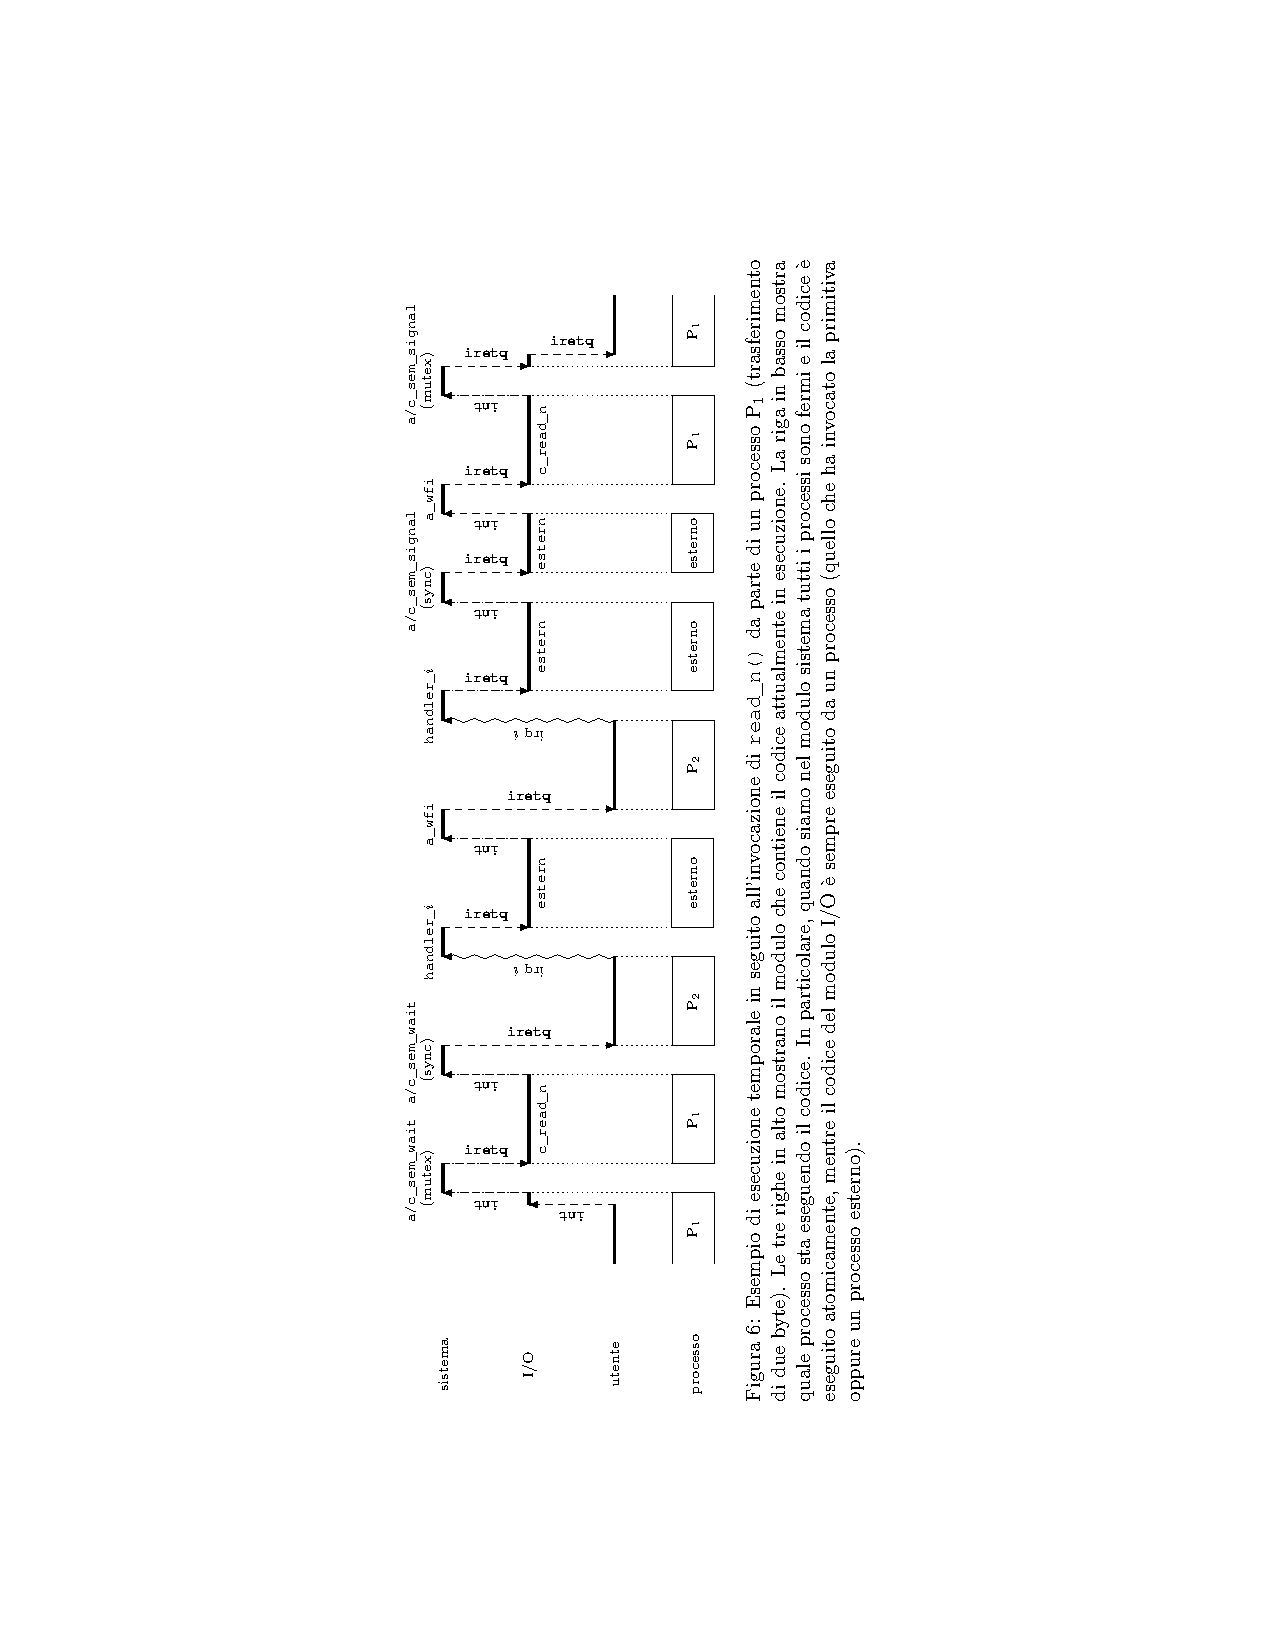
\includepdf[pagecommand={\thispagestyle{plain}},addtotoc={1,subsection,0,{Esempio di esecuzione, passaggio tra i vari moduli},1},pages=-]{pdf/io}

\subsection{Recap} Evidenzio in scuro i moduli eseguiti a livello sistema, mentre tratteggio ciò che viene eseguito con interruzioni abilitate.  
\begin{itemize}
	\item Il modulo I/O è non atomico, ma eseguito a livello sistema.
	\item Il modulo I/O usa primitive fornite dal modulo sistema e fornisce primitive al modulo utente (per esempio quelle di read e write, che fino ad ora abbiamo sempre posto nel modulo sistema). 
\end{itemize}	
\begin{center}
	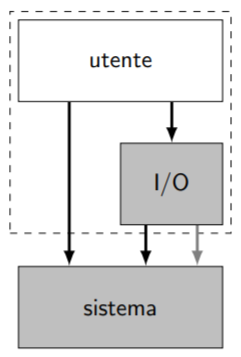
\includegraphics[scale=.7]{img/280.PNG}
\end{center}
\paragraph{Altre primitive sono destinate esclusivamente al modulo I/O}  Possiamo impedirne l'uso da parte del modulo utente impostando la CPL, nelle relative entrate della IDT. La cosa è risolvibile in modo semplice grazie all'esecuzione del modulo I/O a livello di sistema. Le primitive che ci servono nel modulo I/O sono:
\begin{itemize}
	\item \emph{activate$\_$pe};
	\item \emph{wfi};
	\item \emph{gate$\_$init} (per un inserimento controllato nel gate).
\end{itemize}
\clearpage

\section{Primitive per operazioni di bus mastering}
Il nostro sistema offre agli utenti di programmare periferiche bus master. 
\begin{center}
	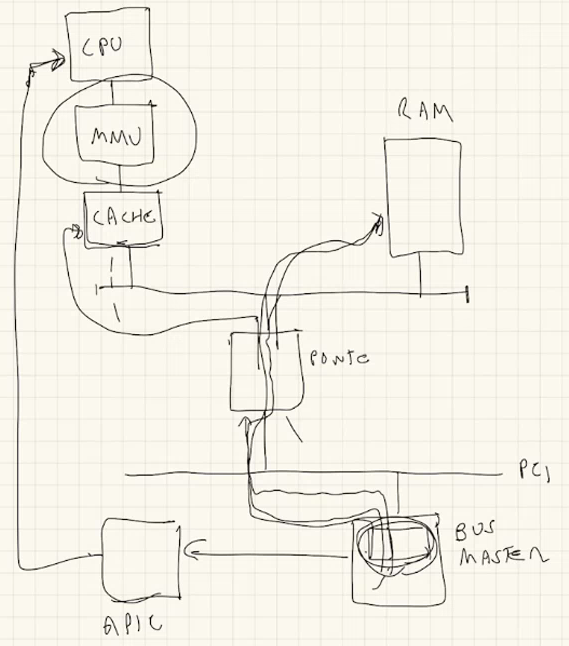
\includegraphics[scale=.6]{img/282.PNG}
\end{center}
Supponiamo di avere primitive di sistema apposite
\begin{verbatim}
	dmaread_m(int id, char* buf, natl quanti)
\end{verbatim}
L'utente specifica una periferica, il buffer, e quanti byte vuole trasferire. L'idea è la stessa dell'operazione non in DMA: In caso di lettura si alloca un buffer, indicando la periferica dalla quale si vuole trasferire. Si tiene conto, anche in questo caso della mutua esclusione
\begin{verbatim}
	wait mutex
	avvia operazione
	wait sync
	rel mutex
\end{verbatim}
Dopo aver avviato l'operazione avremo tutte le cose che abbiamo visto succedere nel bus master, tutto questo mentre la CPU lavora su altro. Quando tutta l'operazione si è conclusa il bus master invia una richiesta di interruzione con l'APIC, segnalando la conclusione dell'intera operazione: a quel punto viene eseguito l'handler. Il processo esterno, grazie alla DMA, ha poco da fare:
\begin{itemize}
	\item segnala al bus master che la richiesta di interruzione è stata gestita (\emph{aknowledge}, lettura di un registro);
	\item rilascia un gettone a sync, risvegliando il processo all'inizio.
\end{itemize}
Queste cose, che potevamo già immaginare, dobbiamo pensarle con la presenza della MMU. 
\subsection{Problemi col bus master}
\begin{itemize}
	\item \textbf{Il bus master non ha a che vedere con la MMU}.
	\begin{itemize}
		\item Per comunicare con la RAM è necessario conoscere l'indirizzo fisico, non c'è storia.
		\item Dobbiamo scorrere l'albero di traduzione e scoprire quale indirizzo fisico è associato all'indirizzo virtuale  \emph{buf}.
		\item \textbf{Primitiva \emph{trasforma}, già vista} Da un punto di vista architetturale siamo nel modulo I/O, quindi possiamo eseguire la primitiva \emph{trasforma}:
		\begin{verbatim}
			paddr trasforma(vaddr v)
		\end{verbatim}
		passo un indirizzo virtuale e ne ottengo uno fisico.
	\end{itemize} 
	\item \textbf{I frame potrebbero essere non contigui}.
	\begin{itemize}
		\item Supponiamo di voler lavorare su un buffer di grandi dimensioni: i frame potrebbero non essere contigui, quindi potrei finire in un frame che non ha nulla a che vedere col buffer.
		\item La soluzione dipende dalla periferica. Potrei creare in memoria una tabella dove si eseguono vari trasferimenti: indico alla periferica dove si trova la periferica (indirizzo fisico), si legge le entrate e ognuna è un indirizzo di trasferimento diverso (con un numero di byte). Indico anche quale sia l'ultima operazioni attraverso un flag. 
		\item Se la periferica non è troppo intelligente allora eseguiamo la cosa in più passi: ogni volta programmo la periferica solo per la parte di trasferimento di un frame. Quando finisce riceviamo un'interruzione e programmiamo un'altra operazione. Ad ogni cambio di pagina chiameremo la \emph{trasforma} per ottenere il corrispondente indirizzo fisico.
		\item \textbf{Requisito opposto rispetto ai trasferimenti non in DMA}.
		
		Nei trasferimenti non in DMA abbiamo detto che è obbligatorio avere il buffer nella parte condivisa. \textbf{Vale la stessa cosa anche con i trasferimenti in DMA?} L'indirizzo del buffer passato alla primitiva non viene utilizzato direttamente, ma tradotto in fisico con la primitiva \emph{trasforma}. A questo punto non è più necessario avere il buffer nella parte condivisa.
	\end{itemize}
\end{itemize}